% rapport.tex

\documentclass[12pt,a4paper]{artikel3}
\usepackage[margin=2cm,head=15pt]{geometry}
\usepackage{isolatin1}
\usepackage[dutch,english]{babel}
\usepackage{lexau}

\input{svnrevision}

\def\thetitle{\LExAu/ Architecture}

\def\Name#1{{\sffamily #1}}
\def\NR#1{(\#\relax #1)}
%###
\def\Paper#1#2{\emph{\href{#2}{#1}\/}\thinspace\footnote{\url{#2}}}
%###

\def\Port/{\emph{port\/}}
\def\PortNR#1{\Port/~\NR{#1}}
\def\IO/{\Name{I\kern .1em/\kern .1emO}}
\def\Actor/{\Name{Actor}}
\def\Encounter/{\Name{Actor}}
\def\Recorder/{\Name{Recorder}}
\def\Optimizer/{\Name{Optimizer}}
\def\Evaluator/{\Name{Evaluator}}

\begin{document}

\thispagestyle{plain}

{\Large\bfseries \thetitle}
\medskip

\begin{tabularx}{\textwidth}{>{\quad\quad\it}lX}
Author&Jeroen van Maanen\\
Revision id.&\SvnRevision/~(\SvnDate/)\\
\end{tabularx}

\section{Context}

In 1996 the author was working in the field of Machine Learning and Kolmogorov Complexity and realized that the model length that is used in the statistical theory of the Minimum Description Length principle can be used to replace the loss function that is used in standard machine learning algorithms.

Standard machine learning algorithms minimize a given loss function that is usually created specifically for a given learning task. Furthermore these learning algorithms need to be trained by giving them the values of the loss function in addition to the interaction with the environment while learning. While these characteristics are convenient and often even desirable, the development of a non-standard algorithm would enrich the field of Machine Learning.

By maximizing the model length instead of minimizing a loss function, it seems possible that a learning algorithm could learn to know an environment just by interacting with it. The \LExAu/ project comprises the design and implementation of such a non-standard learning algorithm. The \LExAu/ algorithm would not require explicit training.

The elegance of this non-standard approach is that the model length is both minimized and maximized. MDL minimizes the sum of the model length and the description length of the data given the model. This places an upper bound on the model length given the data. The rationale for this is that spending more bits on describing the model would put regularities in the model for which there is not enough evidence in the data. Therefore the only way for the \LExAu/ algorithm to make the model grow, is to expose new regularities in the behavior of the environment and prove them. These ideas are described in more detail in \Paper{Model Growth}{http://www.lexau.org/pub/ModelGrowth-final.pdf}, \Paper{Interaction History Tree Models}{http://www.lexau.org/pub/TreeModel-latest.pdf}, and \Paper{Counterfactual Models}{http://www.lexau.org/pub/CounterfactualModel.pdf}.

\section{Goal}

Early versions of \LExAu/ were written in Python, Java, and Clojure. When these attempts progressed, the amount of code related to locking and thread management grew faster than the code related to the algorithm itself. Hopefully this can be avoided in Haskell.

The goal of this project is to realize the principles of \LExAu/ in the form of a Haskell program.

\section{Architecture}

Figure~\ref{fig:architecture} shows the architecture of the Haskell version of \LExAu/.

\begin{figure}[bp]
%###
  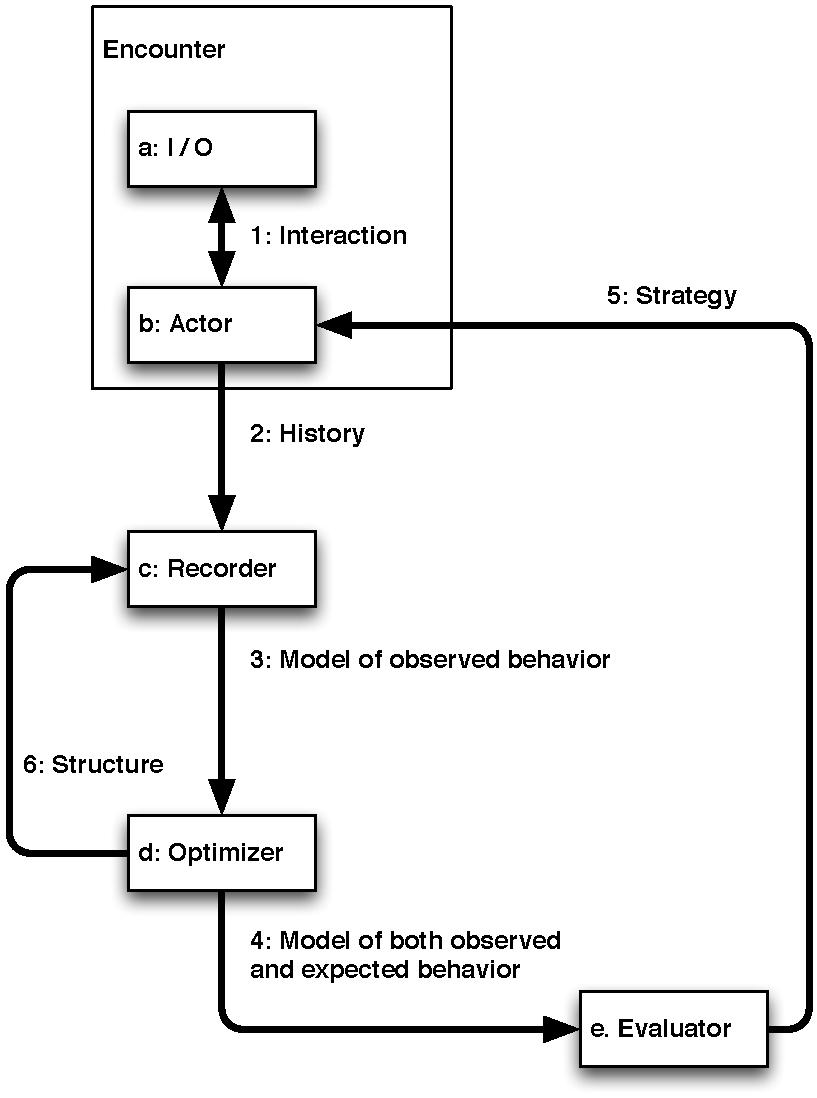
\includegraphics[width=\textwidth]{architecture}
%###
  \caption{Architecture}\label{fig:architecture}
\end{figure}

The algorithm of \LExAu/ is structured as a pipeline of components that communicate with each other through well-defined \Port/s. Each \Port/ represents a stream of messages that are ordered in time. This means that for two messages on the same \Port/ it is always possible to tell which one was sent first. For two messages on \emph{different} \Port/s it may be impossible to determine which one was sent first.

The pipeline starts with an \IO/~component~(a) that has one \Port/: the interaction with the environment~\NR{1}. The interaction with the environment is a bidirectional stream of symbols (the alphabet from which the symbols are taken can be chosen freely for every instantiation of the algorithm and can be either finite of countably infinite).

The second component in the pipeline is an \Actor/~(b) that has three \Port/s: a bidirectional stream of symbols~\NR{1}, strategy updates~\NR{5}, and a unidirectional stream of symbols~\NR{2}. This component uses the latest strategy~\NR{5} to generate output symbols between the input symbols, based on the last few input symbols. The input symbols and the output symbols together allow this component to communicate with the \IO/~component~(a). The \Actor/ component publishes a copy of the exchanged symbols on \PortNR{2}.

The \IO/~component and the \Actor/ are tightly interwoven and implemented as a single Haskell type class. The combination of the \IO/~component and the \Actor/ is called the \Encounter/, because this is the place where \LExAu/ and its environment encounter each other.

The third component in the pipeline is a \Recorder/~(c) that has three \Port/s: a unidirectional stream of symbols~\NR{2}, structure updates~\NR{6} and model updates~\NR{3}. This component updates a model of observed behavior, based on the symbols received on \PortNR{2} and the latest model structure~\NR{6}. The \Recorder/ component publishes updated models of observed behavior on \PortNR{3}.

The fourth component in the pipeline is an \Optimizer/~(d) that has three \Port/s: updates of the model of observed behavior~\NR{3}, updates of the model structure~\NR{6}, and updates of the model of expected behavior~\NR{4}. This component optimizes a model of expected behavior based on the Minimum Description Length principle~(MDL). The \Optimizer/ component publishes model structure updates on \PortNR{6} and publishes the resulting model updates together with the corresponding updated of the model of observed behavior on \PortNR{4}.

The fifth component in the pipeline is an \Evaluator/~(e) that has two \Port/s: updates of the model of both observed and expected behavior~\NR{4} and updates of the strategy~\NR{5}. This component optimizes the strategy based on an autonomous learning criterion. In short, this criterion states: produce output symbols such that the probability of updates on the model of expected behavior is maximized. The \Evaluator/ component publishes the resulting strategy updates on \PortNR{5}.

So \PortNR{5} adds feedback to the pipeline and as a consequence all the number crunching of all components will eventually influence the interaction with the environment.

Together, the combined components and ports form an autonomous, agnostic, generic learning algorithm!

\end{document}
